\documentclass[letterpaper,11pt]{article}

% Packages
\usepackage[utf8]{inputenc}
\usepackage{geometry}
\usepackage{titlesec}
\usepackage{enumitem}
\usepackage{hyperref}
\usepackage{xcolor}
\usepackage{amsmath}
\usepackage{amssymb}
\usepackage{fancyhdr}
\usepackage{graphicx}
\usepackage{float}
\usepackage{booktabs}
\usepackage{tabularx}
\usepackage{listings}
\usepackage{setspace}
\singlespacing

% Page Setup
\geometry{left=2.5cm, right=2.5cm, top=2.5cm, bottom=2.5cm}
\setlength{\headheight}{14pt}
\pagestyle{fancy}
\fancyhf{}
\rhead{\textbf{Final Report}}
\lhead{01 - CP683-BF - 4/2026}
\cfoot{\thepage}

% Custom Colors
\definecolor{primary}{RGB}{0, 51, 102}
\definecolor{accent}{RGB}{204, 0, 0}

% Title Format
\titleformat{\section}
{\normalfont\Large\bfseries\color{primary}}{\thesection}{1em}{}

\titleformat{\subsection}
{\normalfont\large\bfseries\color{primary}}{\thesubsection}{1em}{}

% Code listing style
\lstdefinestyle{code}{
    backgroundcolor=\color{gray!8},
    basicstyle=\ttfamily\small,
    keywordstyle=\color{blue},
    commentstyle=\color{gray},
    stringstyle=\color{teal},
    breaklines=true,
    frame=single,
    numbers=left,
    numberstyle=\tiny\color{gray},
    tabsize=2
}
\lstset{style=code}

% Metadata
\title{\textbf{AIVS: Anonymous Identification Verification System}\\Based on Ring Signatures with Isolated Smart Card Hardware}
\author{
\textit{Dinh Anh Khoa Nguyen - 245849840 - nguy9840@mylaurier.ca}\\
\textit{Jiangtao Wang - 245823800 - Wang2370@mylaurier.ca}\\
\textit{Leila Chen - 245850620 - chen5062@mylaurier.ca}\\
\textit{Yuyang Wu - 245817310 - wuxx7310@mylaurier.ca}\\
}
\date{April 2026}

\begin{document}

\maketitle
\thispagestyle{empty}

\begin{abstract}
    This report outlines the engineering implementation of a privacy-preserving messaging platform that decouples message integrity from identity revelation. Leveraging Yubikey hardware PRF and nested Ring Signatures, the system allows users to send undeniable, tamper-proof messages anonymously, with the exclusive capability to retroactively prove authorship. The project adopts an Agile methodology, utilizing React/TypeScript for the frontend and Node.js for the backend.
\end{abstract}

\newpage

% ============================================================
\section{Evaluation}

\subsection{Functional Testing}
Functional testing was conducted to evaluate whether the prototype correctly supports the intended end-to-end workflow, including authentication, anonymous message creation, message-pack management, and authorship confirmation. The purpose of this evaluation was not to assess user interface quality in isolation, but to verify that the frontend, backend, and client-side cryptographic components operate consistently as an integrated system.

The first group of tests focused on the WebAuthn-based login flow. A user was able to initiate registration or authentication challenges from the browser, complete credential operations with the hardware token, and obtain a valid session for subsequent requests. After successful login, the client correctly restored the authenticated state and exposed the corresponding user functions, indicating that challenge handling, session issuance, and session recovery were workflow-level functional successes.

\begin{figure}[H]
    \centering
    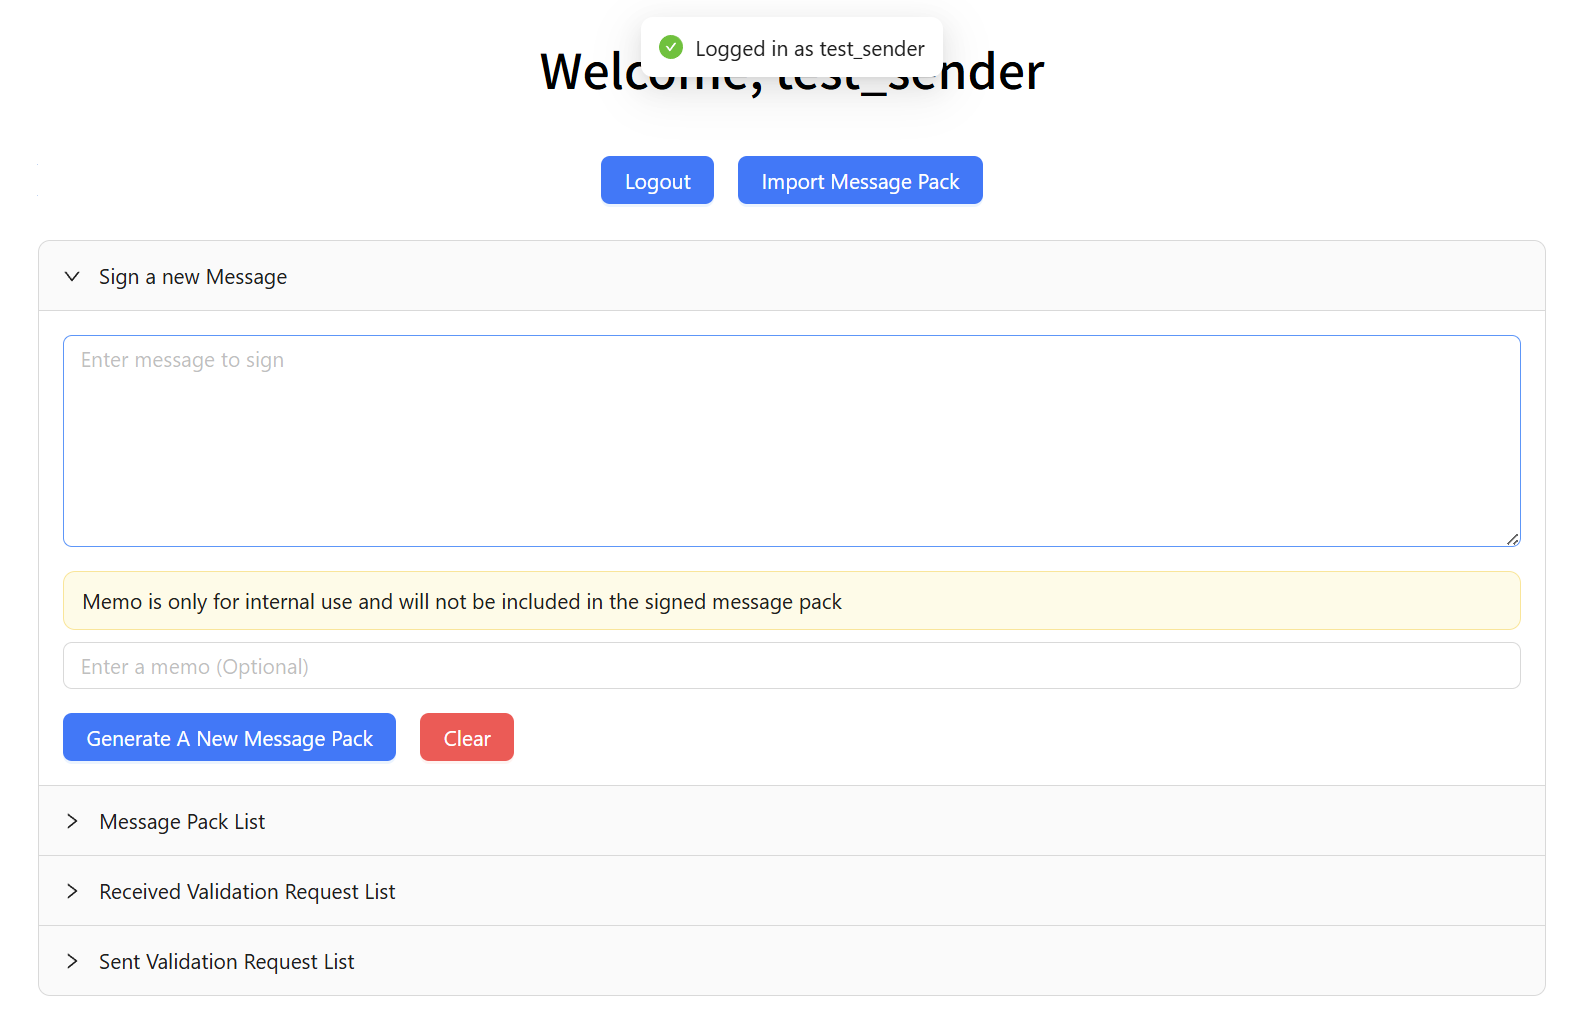
\includegraphics[width=0.70\textwidth]{functional-login-success.png}
    \caption{Authenticated user interface after successful login and session establishment.}
\end{figure}

The second group of tests examined anonymous message-pack generation and storage. After authentication, the client successfully derived a one-time key with the participation of the YubiKey PRF, generated the corresponding ring-signature-based message pack locally, and submitted the serialized result to the backend. The stored message pack could then be retrieved and displayed in the message list, confirming that local cryptographic generation, backend persistence, and frontend rendering were correctly connected.

\begin{figure}[H]
    \centering
    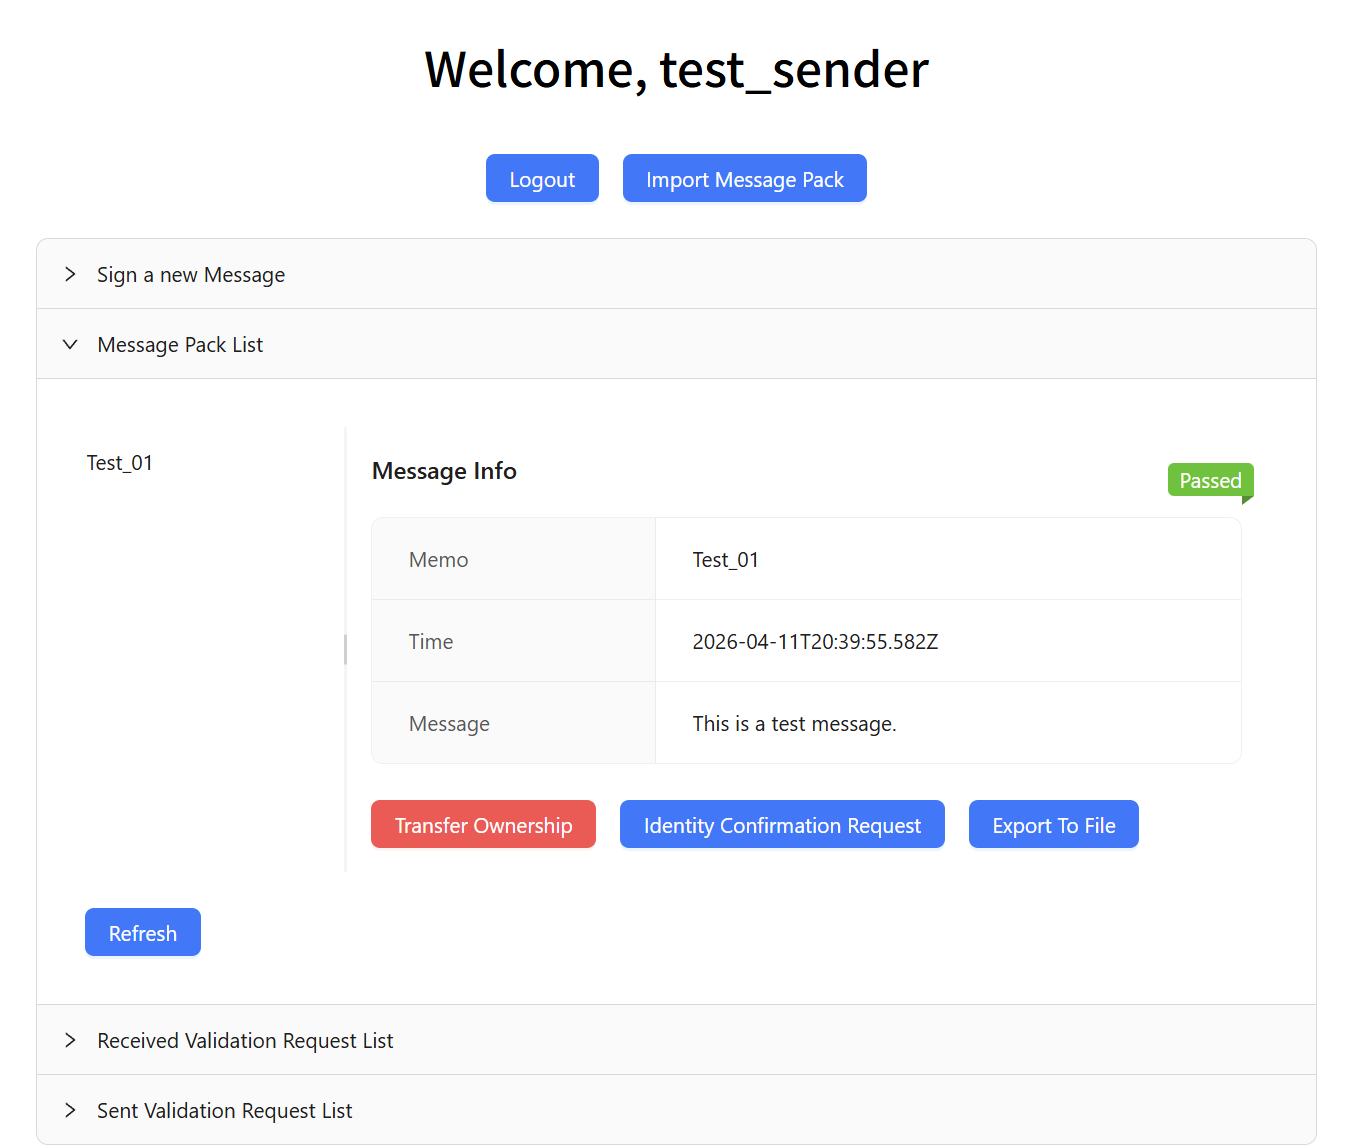
\includegraphics[width=0.70\textwidth]{functional-message-pack.png}
    \caption{Stored message pack displayed in the list with management actions.}
\end{figure}

Additional tests covered message-pack management and the authorship confirmation workflow. A user could export a stored message pack, transfer its ownership to another user, and observe the updated ownership state after refreshing the list. Furthermore, a recipient could initiate a validation request, the claimed sender could respond with a proof derived from the original credential, and the requester could obtain a final validation status. These results indicate that the prototype already supports the complete functional loop from anonymous message creation to later identity revelation.

\begin{figure}[H]
    \centering
    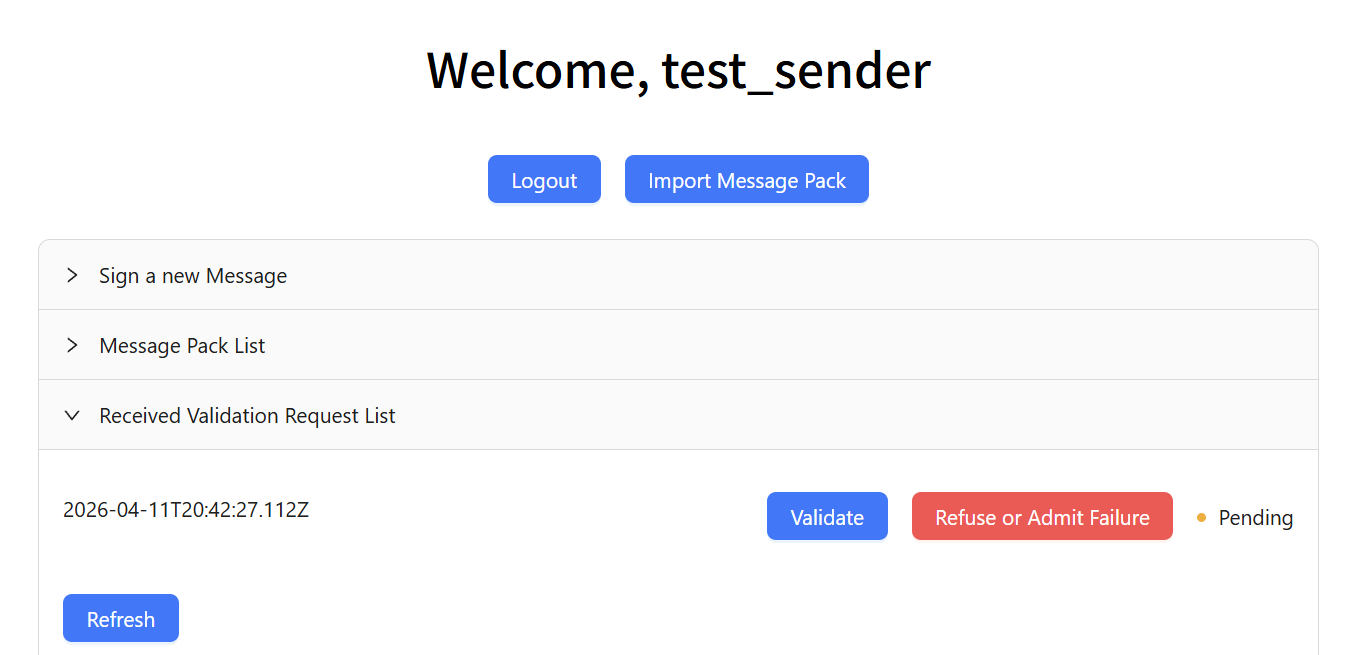
\includegraphics[width=0.70\textwidth]{functional-validation-received.png}
    \caption{Received validation request shown in the pending state before proof handling.}
\end{figure}

\begin{figure}[H]
    \centering
    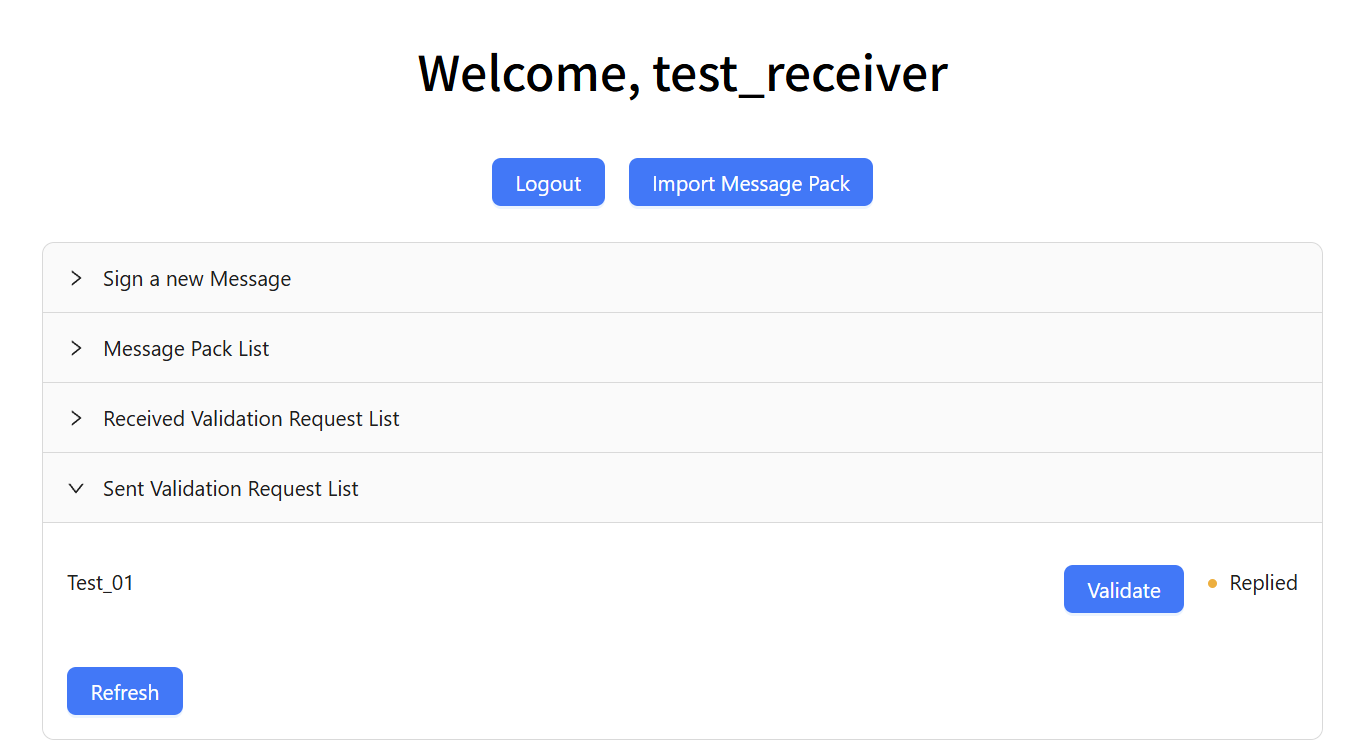
\includegraphics[width=0.70\textwidth]{functional-validation-replied.png}
    \caption{Sent validation request shown after the responder has returned a proof.}
\end{figure}

\subsection{Security Analysis}
The security properties of the prototype are primarily derived from the combination of client-side cryptographic execution, hardware-assisted key derivation, and the two-layer ring-signature construction. Instead of directly signing messages with a long-term identity key, the system derives a one-time key with the participation of the YubiKey through the WebAuthn PRF extension. As a result, message authenticity can be established without introducing a direct and persistent link between signed content and the user's long-term identity. 

First, the system supports anonymous authenticity. The outer ring signature allows a recipient to verify that a message was produced by a valid member of the ring without revealing which member actually signed it. Because each message is associated with a freshly derived one-time key and a set of decoy public keys, signatures are not directly tied to a stable long-term identity.

Second, the prototype supports controlled authorship revelation. In addition to the outer signature, the sender generates an inner ring signature and protects it as an encrypted proof derived from the same hardware-backed credential. This allows the sender to later provide additional cryptographic evidence and confirm authorship when needed.

Third, the backend does not store private signing material and does not perform the cryptographic operations required to generate or reveal proofs. Its role is limited to challenge management, session handling, message-pack storage, and validation-request coordination. As a result, the server is not required to act as a trusted identity escrow for the messaging workflow.

Overall, the prototype demonstrates that anonymous transmission, integrity verification, and later authorship confirmation can coexist within one browser-based workflow.

\subsection{Performance Analysis}
Functional testing and backend API timing observations were conducted through the online test environment at \texttt{https://cp683.ryonanamizu.com/}. The system was accessed through a web browser, and browser developer tools were used to inspect request timing for representative backend endpoints. Cryptographic performance measurements, by contrast, were collected through a separate local benchmark that focused on client-side ring-signature generation, verification, message-pack construction, and proof revelation.

\begin{table}[H]
    \centering
    \begin{tabular}{lccc}
        \toprule
        Metric                           & Mean (ms) & Min (ms) & Max (ms) \\
        \midrule
        LRS generation                  & 39.34     & 37.19    & 45.96    \\
        LRS verification                & 38.81     & 37.12    & 44.11    \\
        Approx. message pack generation & 77.71     & 75.15    & 85.28    \\
        Approx. proof revelation        & 0.96      & 0.39     & 2.68     \\
        \bottomrule
    \end{tabular}
    \caption{Local benchmark results for the default configuration with ring size 8.}
\end{table}

Under the default configuration with \texttt{ring size = 8}, each metric was measured over 20 runs in the local benchmark. The results show that LRS generation and verification required 39.34 ms and 38.81 ms on average, respectively. Approximate message-pack generation was the most expensive measured client-side step at 77.71 ms, while approximate proof revelation was the lowest-cost step at 0.96 ms.

As a supplementary observation, several backend API latencies were also inspected through browser developer tools. Under the local deployment setup, \texttt{POST} \path{/message}, \texttt{GET} \path{/message/list/by\_username/:username}, and \texttt{POST} \path{/validation-requests} required approximately 66.57 ms, 53.44 ms, and 47.61 ms, respectively.

Overall, the measurements indicate that the main runtime cost of the prototype lies in local cryptographic processing, especially full message-pack construction.

\subsection{Limitations and Edge Cases}
Although the prototype demonstrates the engineering feasibility of anonymous messaging, public verification, and later authorship revelation, several limitations and edge cases remain and should be considered when interpreting the evaluation results.

First, the current system is still a research prototype. Although the frontend supports browser-based registration and authentication flows, server-side attestation verification during registration and assertion verification during login are not yet fully implemented.

Second, the design depends on hardware and platform support for the WebAuthn PRF extension. If the authenticator or browser does not support this capability, one-time key derivation and proof decryption cannot proceed as intended.

Third, the anonymity-set size is fixed in the current implementation. The default configuration uses a 1-of-8 ring, which is sufficient for prototype validation but does not represent a flexible or production-oriented anonymity setting.

Lastly, the core cryptographic workflow is executed in the browser, so security still depends in part on the integrity of the client environment. In addition, loss of the original hardware token prevents later authorship revelation, and application metadata may still introduce correlation risks.

In conclusion, these limitations show that the current contribution of the project is to validate mechanism feasibility rather than to provide a production-ready deployment.

% ============================================================
\newpage
\bibliographystyle{plain}
\begin{thebibliography}{9}

\bibitem{noether2015}
Shen Noether,
\newblock Ring Signature Confidential Transactions for Monero,
\newblock Cryptology {ePrint} Archive, Paper 2015/1098, 2015.
\newblock Available at \url{https://eprint.iacr.org/2015/1098}

\bibitem{webauthn3}
Tim Cappalli, Michael B. Jones, Akshay Kumar, Emil Lundberg, and Matthew Miller,
\newblock {Web Authentication: An API for accessing Public Key Credentials - Level 3},
\newblock W3C Candidate Recommendation Snapshot, January 2026.
\newblock Available at \url{https://www.w3.org/TR/webauthn-3/}

\end{thebibliography}

% ============================================================

\end{document}
